\section{\xxx Overview} \label{sec:overview}

\xxx is deployed as a typical \smr system. A set of three or five replicas is 
set up within a LAN, and each replica runs an \xxx instance containing the 
same server program. On the \xxx system starts, one replica becomes the 
\emph{primary} (or leader) replica which proposes the order of requests to 
execute, and the others become backup replicas which follow the primary's 
proposals. A number of clients in LAN or WAN send network requests 
to the primary and get responses.  If the primary machine fails, the other 
replicas run a leader election~\cite{paxos:practical} to elect a new primary.

This section first presents \xxx's architecture, including its consensus 
interface and a \xxx instance's main components, and then uses an 
example to show how \xxx works with server programs.

% \subsection{Usage} \label{sec:usage}
% TBD.

\subsection{Architecture} \label{sec:abstraction}

To support general server programs transparently, \xxx chooses the POSIX socket 
API as its consensus interface. \xxx enforces two kinds of orders for socket
calls. First, for client programs' out going socket calls (\eg, \connect and
\send), \xxx enforces that all replicas see the same sequence of client socket 
calls with \paxos. \xxx does not need to order the clients' 
blocking socket calls because \xxx is not designed to replicate clients. 
Second, for a server program's blocking socket calls (\eg, \poll, \accept, and 
\recv), \xxx enforces that these calls are scheduled and 
returned in the same sequence of logical times across replicas. \xxx 
responses to the clients only using the server program on the primary, and it 
drops the responses of the server programs on backups.

For a server program's outgoing socket calls (\eg, \send), \xxx simply 
schedules them using \dmt and does not invoke consensus. The 
reason is that these calls readily have consistent contents via enforcing 
the same logical admission times of input requests and the same thread 
schedules for server programs across replicas.

\begin{figure}[t]
\centering
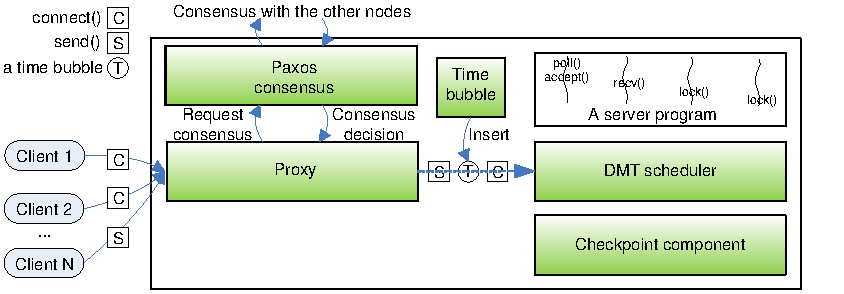
\includegraphics[width=.5\textwidth]{figures/repbox}
% \vspace{-.20in}
\caption{{\em The \xxx Architecture.} \xxx components are shaded (and in
  green).} \label{fig:repbox}
\vspace{-.05in}
\end{figure}

Figure~\ref{fig:repbox} shows a \xxx instance running on the primary. The 
instance contains five main components, the proxy, the 
\paxos consensus, the \dmt scheduler, the \timealgo component that enforces the 
same logical clocks for servers' blocking socket calls across
replicas via inserting time bubbles, and the checkpoint component that 
periodically checkpoints the server program. A server program runs 
transparently in a \xxx instance without being aware of \xxx's components. A 
backup replica runs the same \xxx instance except that its proxy does not 
accept connections from clients and does not invoke consensus.

%% Each component.
The proxy component is a \xxx instance's gateway.  It accepts socket
requests from clients and forwards the requests to the server program on its 
own replica. It accepts responses from the server program and forwards the 
responses to the clients. Once the proxy receives a
client socket request, it invokes the \paxos consensus component running
on its own replica for this request.  The proxy does not block-wait for 
this decision which may take a while to reach. Once the proxy is notified by 
the \paxos component that some requests' decisions are made, it forwards the 
requests in decision order to the server program.

The \paxos consensus component is a \paxos protocol that receives a client 
socket request from its own proxy and invokes a consensus process on
this request.  This component is also the only \xxx component that
communicates among different replicas. \xxx's \paxos implementation is 
based on a well-known and concise protocol~\cite{paxos:practical}. After
\xxx's \paxos components reach consensus on a client socket call, each \paxos 
component notifies its own proxy to forward this call to its server program.

The \dmt component runs within the server program's process. \xxx leverages 
\parrot~\cite{parrot:sosp13} as the \dmt scheduler because \parrot 
runs fast on a wide range of 108 popular multithreaded programs. Specifically, 
\parrot uses a runtime technique called \ldpreload to dynamically intercept 
\pthread synchronizations (\eg, \mutexlock) issued by an executable and 
enforces a well-define, round-robin schedule on these synchronization 
operations for all threads, practically eliminating nondeterminism in thread 
synchronizations.

Although \parrot is not designed to resolve data races
deterministically, \xxx's replication tolerates data races that have
fail-stop consequences, and can further catch the
other data races by running a race detector on a backup replica (see
\S\ref{sec:limit}).  \xxx augments the \dmt component to schedule the
return points of socket calls in server replicas, too, to ensure that
requests are admitted at consistent logical times across replicas.

The \timealgo component sits between the proxy and the \dmt's processes, and it 
is invoked on two conditions. First, on a server's bootstraps, \xxx invokes 
time bubble insertions to make sure that the server programs across replicas 
reach the same initial state and wait for the first input request. Second, if 
the \dmt component has not received any input request from the proxy for a 
physical duration \ntimeout, a time bubble insertion is invoked as the boundary 
of two request bursts. To ensure the same sequence of inserted time bubbles 
across replicas, the same \paxos consensus as that for client socket calls is 
invoked. For each time bubble, each replica's \dmt scheduler promises to run a 
number of \nclock synchronizations and not to admit any 
client socket call.

If the \dmt scheduler exhausts the logical clocks in a time bubble, it either 
admits new client socket call (if any) or inserts another time bubble. If the 
scheduler does not exhaust the logical clocks after serving current requests, 
\parrot has a mechanism to exhaust them rapidly. More discussions on the values 
of the two parameters \ntimeout and \nclock are given in 
\S\ref{sec:sensitivity}.



To recover from replica failures or add new replicas, the checkpoint 
component is invoked every minute on a backup replica. It
checkpoints the server process running with \dmt.  While one can always start a 
server replica from scratch and replay the entire sequence of socket calls, 
this replay can be extremely time-consuming for long-running servers.  Prior 
\smr systems rely on narrow state machine interfaces for checkpoint and
recovery, which does not work for general server programs. Instead, \xxx
leverages two popular open source tools: \criu, to checkpoint process 
state such as CPU registers and memory; and \lxc, to checkpoint the file 
system state of a server program's current working directory and installation 
directory.

Each checkpoint in \xxx is associated with a global index in \paxos's consensus 
order, so if one replica needs recovery, \xxx ships the latest checkpoint from a 
backup replica, restores the process running \dmt and the server program, and 
re-executes socket calls starting from this index. The proxy and consensus 
components do not require checkpoints because we explicitly designed their 
execution states independent to the server's process.


\subsection{Assumptions} \label{sec:limit}

\xxx leverages \parrot to make synchronizations deterministic.  \parrot is
explicitly designed not to handle data races. However, in the context of \xxx,
data races are less harmful because, if they cause backups to crash, \xxx
can still operate and recover as long as a quorum of the replicas is
still alive. Moreover, leveraging \xxx's replication architecture, one can 
deploy a race detector on a backup replica~\cite{repframe:apsys15}, achieving 
both good \xxx performance and full determinism.

There are other sources of nondeterminism besides thread scheduling and
request timing.  These other sources of nondeterminism may cause backups
to diverge, too.  For example, backups may do different things based on
their IP addresses, data read from \v{/dev/random}, addresses returned by
\v{malloc}, physical time observed via \v{gettimeofday}, or delivery time
of signals.  Prior work has shown how to eliminate these sources of
nondeterminism using record-replay~\cite{scribe:sigmetrics2010, 
respec:asplos10} or OS-level techniques~\cite{dos:osdi10}, which \xxx can 
leverage.  Another solution is to treat all these sources as inputs and 
leverage distributed consensus to let all replicas observe the same input.  We 
leave these ideas for future work. We inspected server 
programs' network outputs among replicas, and we found that these outputs 
were consistent in \xxx except physical times (\S\ref{sec:correctness}).

For a server program that spawns multiple processes which communicate via
IPC, \xxx currently does not make these IPC operations deterministic.  We
expect that it should be easy to support deterministic IPC in \xxx because it
already makes socket API deterministic.  In addition,
dOS~\cite{dos:osdi10} and DDOS~\cite{ddos:asplos13} have many effective
techniques for tackling this problem, which \xxx can leverage.

